\documentclass[11pt,a4paper]{article}
\usepackage[left=15mm,right=15mm,top=15mm,bottom=15mm]{geometry}
\usepackage{graphicx,musicography}
\title{PianoScript}
\author{a piano-roll music notation format}
\date{}

\begin{document}

\maketitle

\begin{center}

\includegraphics[width=.27\textwidth]{images/moonlight.jpg}
\end{center}

\newpage

\tableofcontents

\newpage

\section{Introduction; what is PianoScript and why?}
PianoScript is a music notation for pianists that like to read music visually and practically. The main goal is to provide a tool that plots the rhythm and harmony of a midi-file in a readable way as a music notation including accents, dynamics in several ways, text and more elements.\\

PianoScript is based/inspired by an almost hundred-year-old music notation called Klavarskribo\footnote{Look on www.klavarskribo.eu for more information.}. There are a small number of eye-catching visual differences that make PianoScript a different music notation. Unlike Klavarskribo, PianoScript is only aiming for piano music/players.\\

The main reason PianoScript was born is that Philip Bergwerf discovered Klavarskribo and began searching for improvements and different possibilities in terms of visual design as well the practical readability of the notation itself. In this process, Philip formed the idea of plotting a midi-file over the klavarskribo staff in the form of grey midi-notes.\\

%------------------------------------------------------------
\pagebreak
\part{The PianoScript music notation explained}
\section{Introduction}
PianoScript is a readable piano-roll-editor that can be printed paper. Take a look at the guitar-tab. PianoScript is essentially a real piano-tab!

PianoScript can be read from left to right or from top to bottom. The reader can choose to read horizontally or vertically. The advantage of reading vertically is that the orientation of the notation is the same as the orientation of the instrument you are playing. For extra clarity, we only explain everything in the horizontal orientation.

\subsection{Pitch on a twelve-tone staff} 
Pitch is expressed on a twelve-tone staff. As you can see on the first page of this document, the staff exists from groups of two and three lines that are connected to a miniature piano keyboard and thus, are the black keys.

\begin{center}
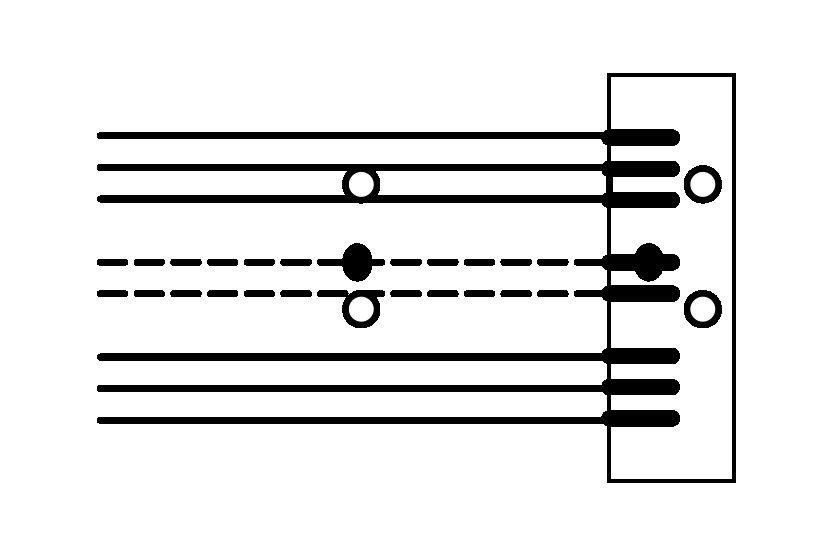
\includegraphics[scale=1]{images/cminor.jpg}\\
\emph{\small picture 1: a c minor chord on the PianoScript staff} 
\end{center}


The notes are black or white depending on the color of the piano key. This means that all black notes are on top of a staff line while all white notes are in between or 'glued to' a staff line.

The staff is at least as large as the range of the music. A rule is that the dashed lines are always visible because it is the clef.

\subsection{Clef}
The clef is represented as a group of two c\musSharp/d\musFlat \space and d\musSharp/e\musFlat\space lines. We call them \emph{\textbf{the central lines}}. They give the position of the central-c; the c that is in front of you in the middle of the piano keyboard.

You can find the right note in the right octave relative to the central lines. The central lines are always visible. An empty measure shows only the clef.

\subsection{Rhythm}
\subsubsection{Midi-notes}
Rhythm is expressed in distance like in a piano-roll editor or inside 'Synthesia' youtube videos. A piano-roll has 'midi notes' that are displaying the rhythmic information of a midi-file. The most important for reading rhythm is to have a clear starting point and end point for every note. The \underline{stem} of the note is used to point out the exact point in time the note starts. The \underline{note stop} is a small vertical black dash + the grey midi note stops on that point.

\subsubsection{Base grid and manual grid}
There is a base grid that points out the obvious beats from the time signature. In a lot of cases, we need more grid lines to clarify the rhythm. We call them the manual grid. The visual difference is that the base grid spans the whole staff height and the manual grid is a finer dashed partially spanned line that usually highlights half of a beat if necessary. The manual grid is manually added by the typesetter.

\subsubsection{Example: moonlight sonata, first bar}
\begin{center}
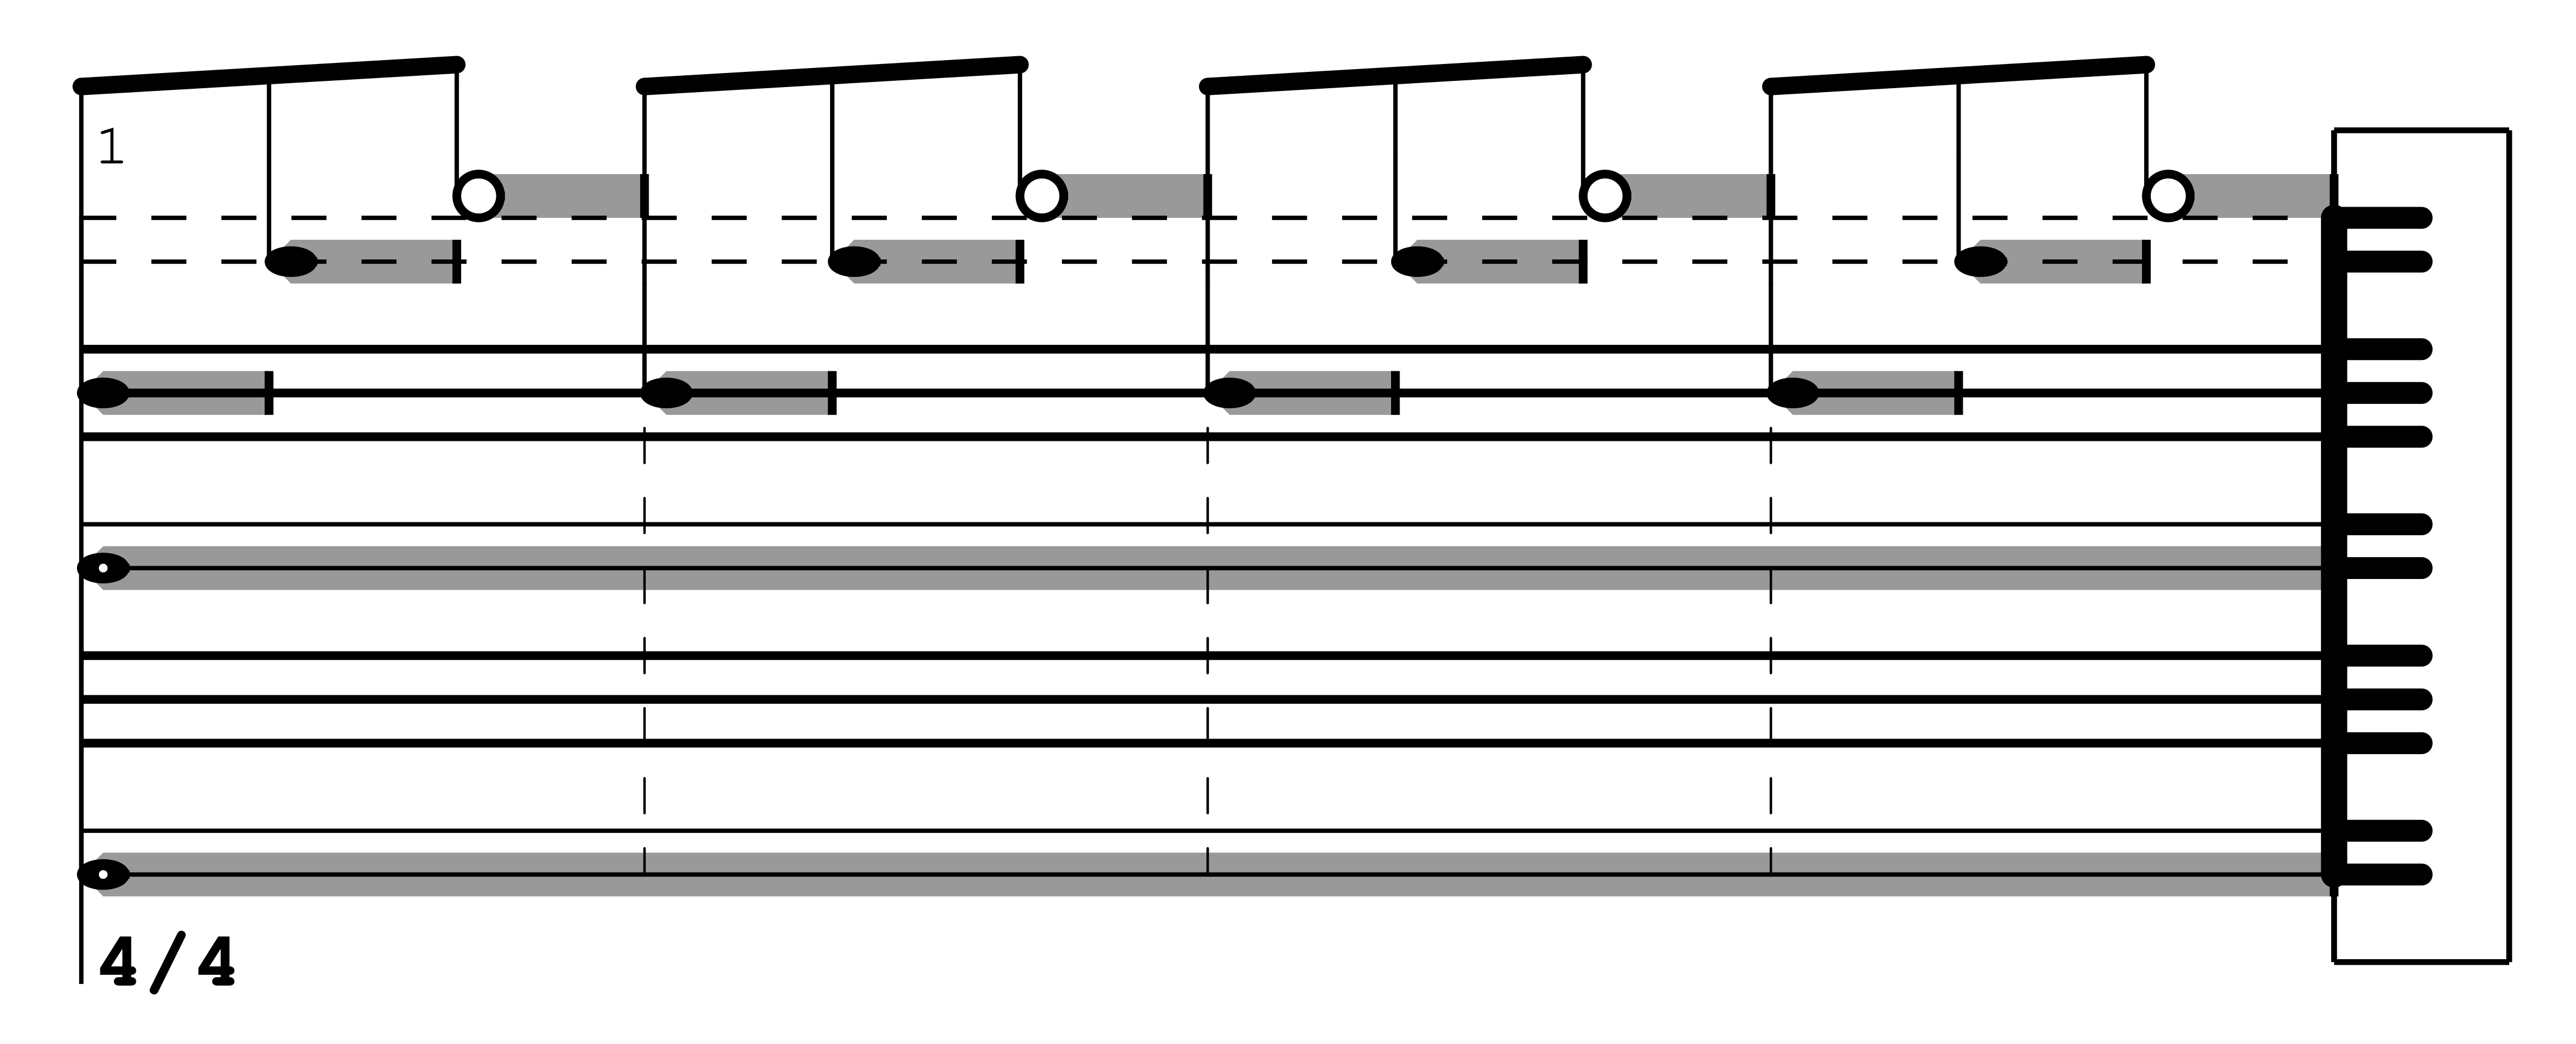
\includegraphics[scale=1]{images/moonlightonebar.jpg}\\
\emph{\small picture 2: the first bar of the moonlight sonata} 
\end{center}

This example bar is written in a 4/4 time signature. We divide the length of the bar into four equal pieces and thus every 'grid space' is one \underline{quarter} note long. This is the \emph{base-grid}.

If we follow the logic of relatively reading the rhythm: There are two notes with a duration of a \underline{whole} note(four quarter spaces = whole note). The grouped notes on the upper side are all an equal length. There fit three notes in a quarter grid space so these are \underline{quarter triplets}.

\subsubsection{Grouping of notes}
Optionally we can group notes to give an overview of the rhythmic information using a beam. A beam looks like an eight-beamed beam from traditional music notation but has nothing to do with length. Usually, we group all notes that are inside the base grid but depending on the situation the beam grouping may differ.

\subsection{Hand}
You can read for which hand the note is written in two ways:
\begin{itemize}
\item{The left-hand notes do have a tiny dot inside the note. The right-hand notes don't have a dot inside the note.}
\item{If the stem points down the hand is left. If the stem points up the hand is right.}
\end{itemize}

%------------------------------------------------------------
\section{Discussing different elements and techniques}
\subsection{Ornaments}
Roughly there are two types of notes:
\begin{itemize}
\item{normal notes that point out the basic rhythm of the music}
\item{ornaments or decoration notes}
\end{itemize}

In traditional music notation, many symbols represent all kinds of ornaments. Because PianoScript is a performance notation(it's a midi-file representation suitable for printing and reading on a piece of paper), the best way to write ornaments is to write them literally. 

To make it clear we are writing an ornament, we write ornaments without a stem. Ornaments are in general meant like a roughly timed note or group of notes; it leaves a lot of interpretation for the pianist. Therefore it doesn't bother if the rhythmic notation is less clear because of the absence of the stem, it still gives a clear guideline on how to play the ornament.

\subsubsection{Arpeggio}
\begin{center}
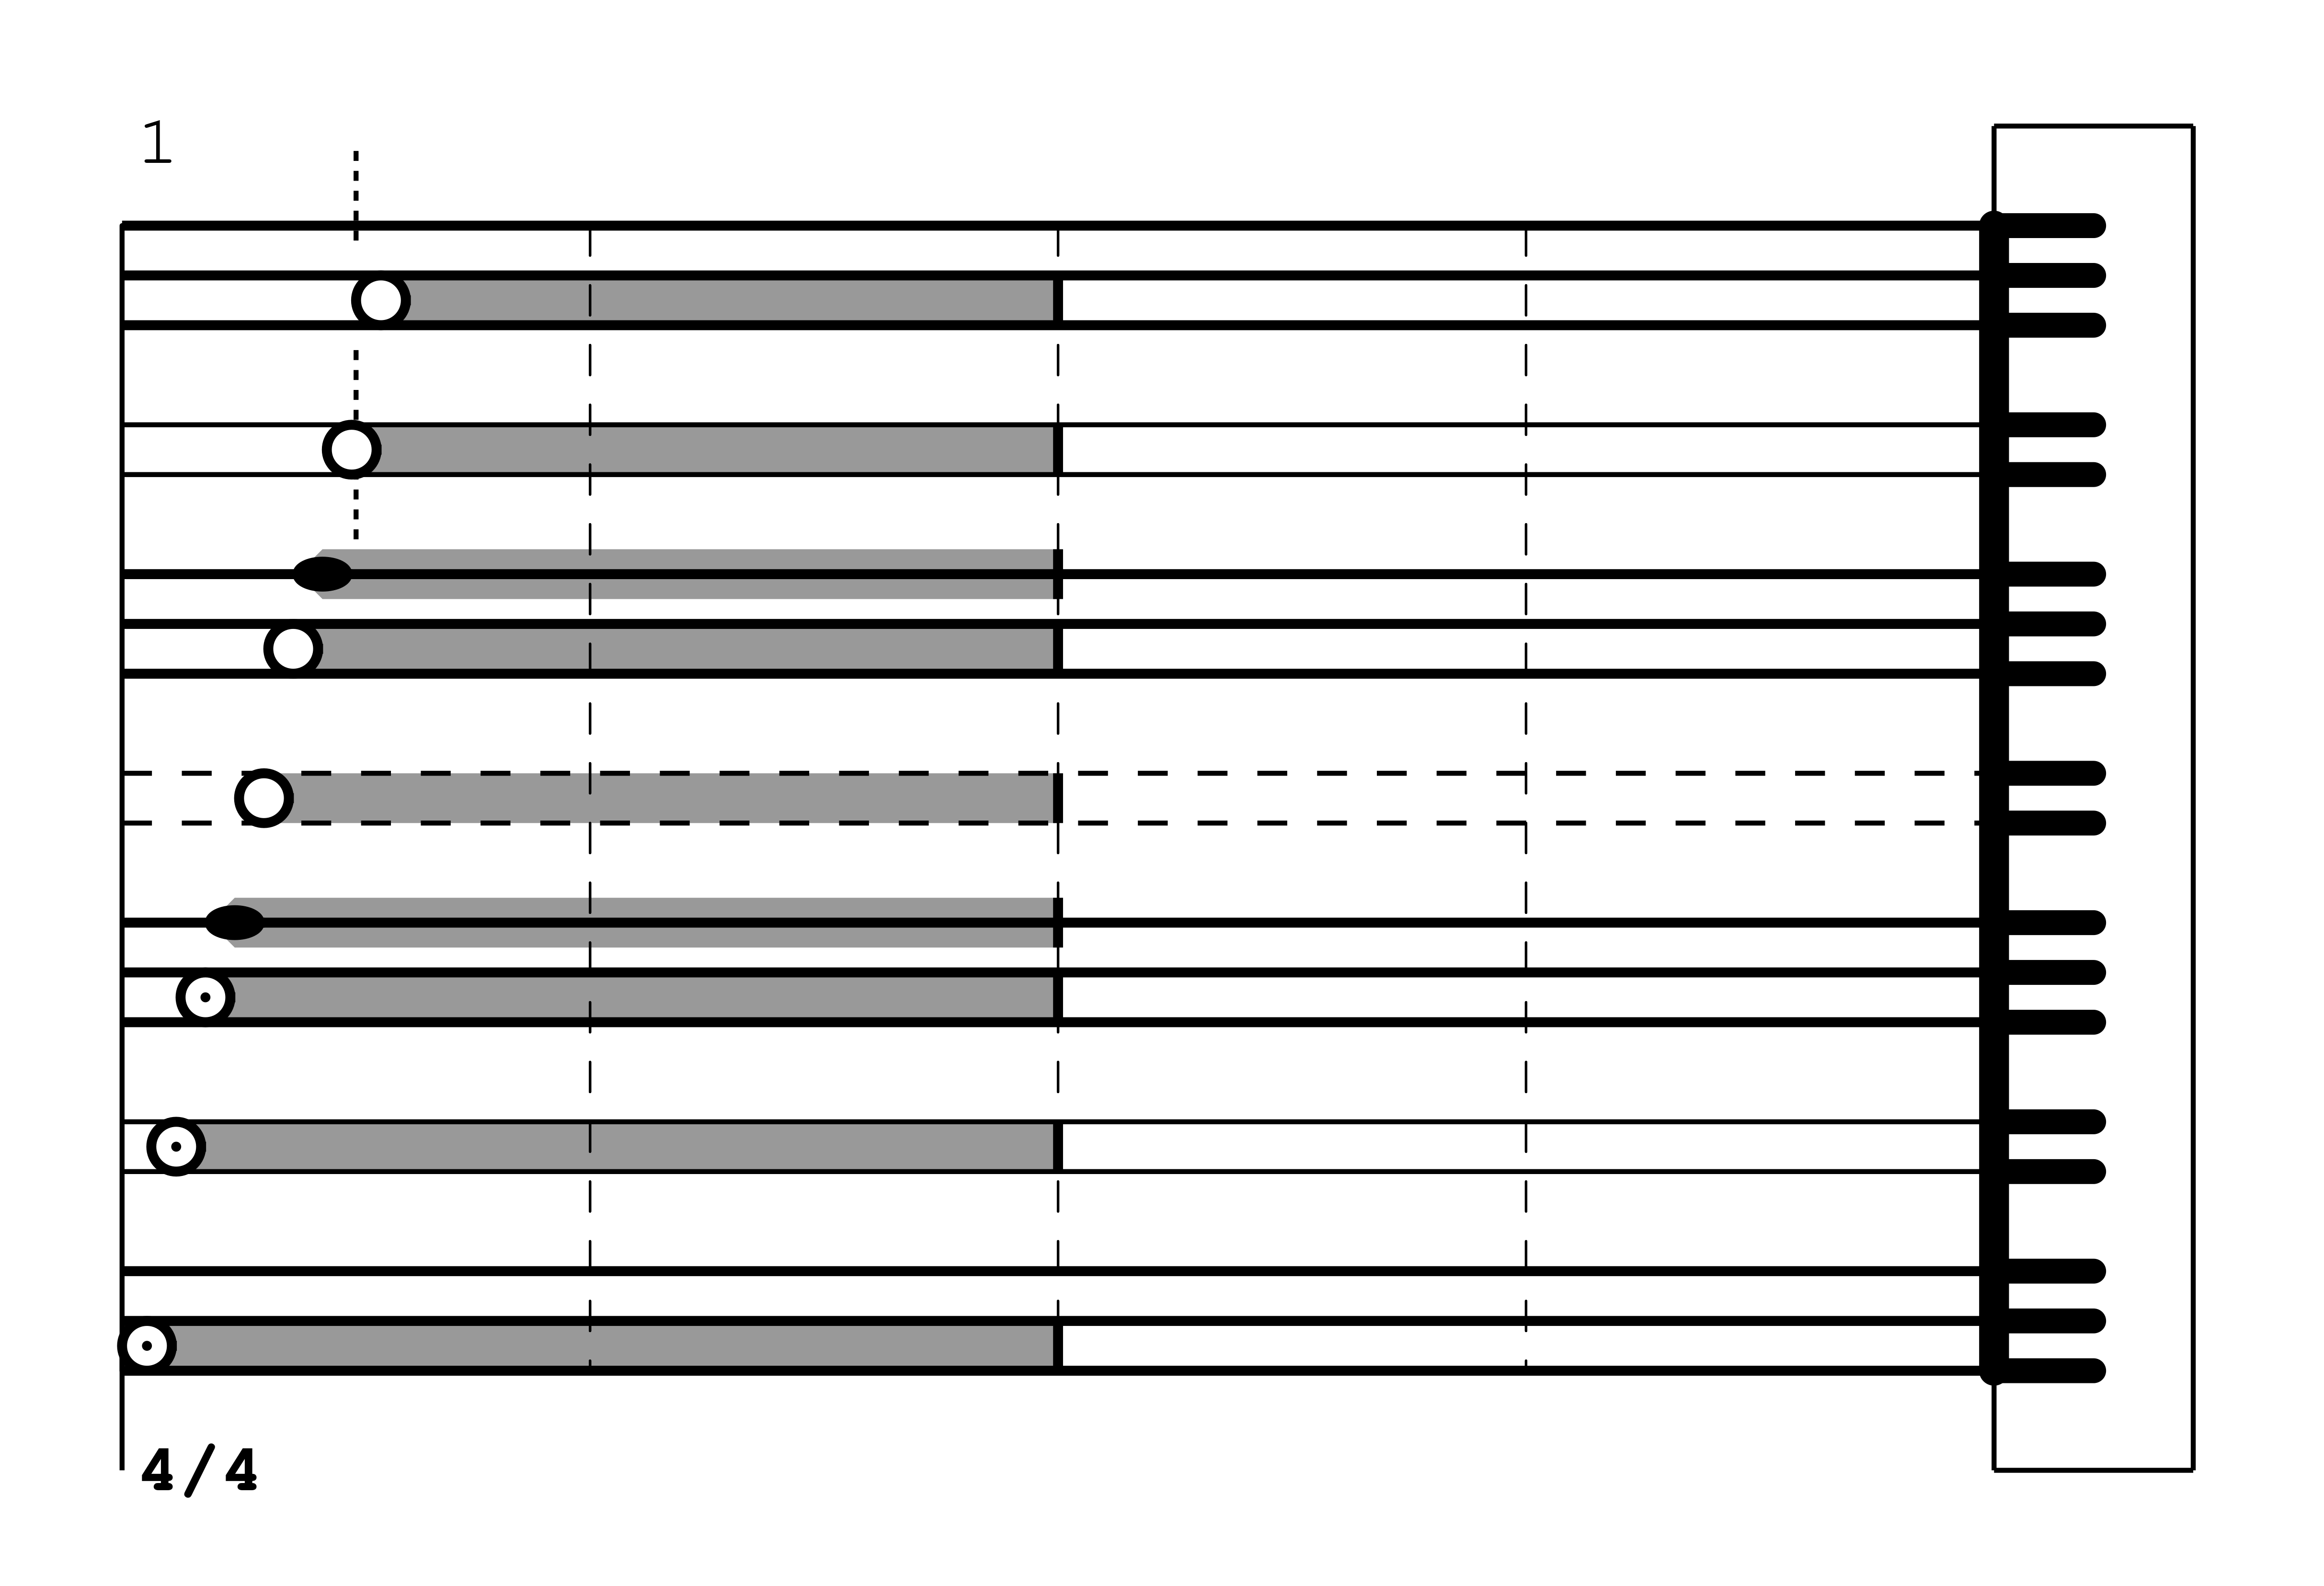
\includegraphics[scale=.75]{images/arpeggio.jpg}\\
\emph{\small picture 3: example of an arpeggio}
\end{center}

In this example we see also for the first time a manual grid applied to point out where the arpeggio ends; so this arpeggio spans an eight-note value.

\subsubsection{Trill}
\begin{center}
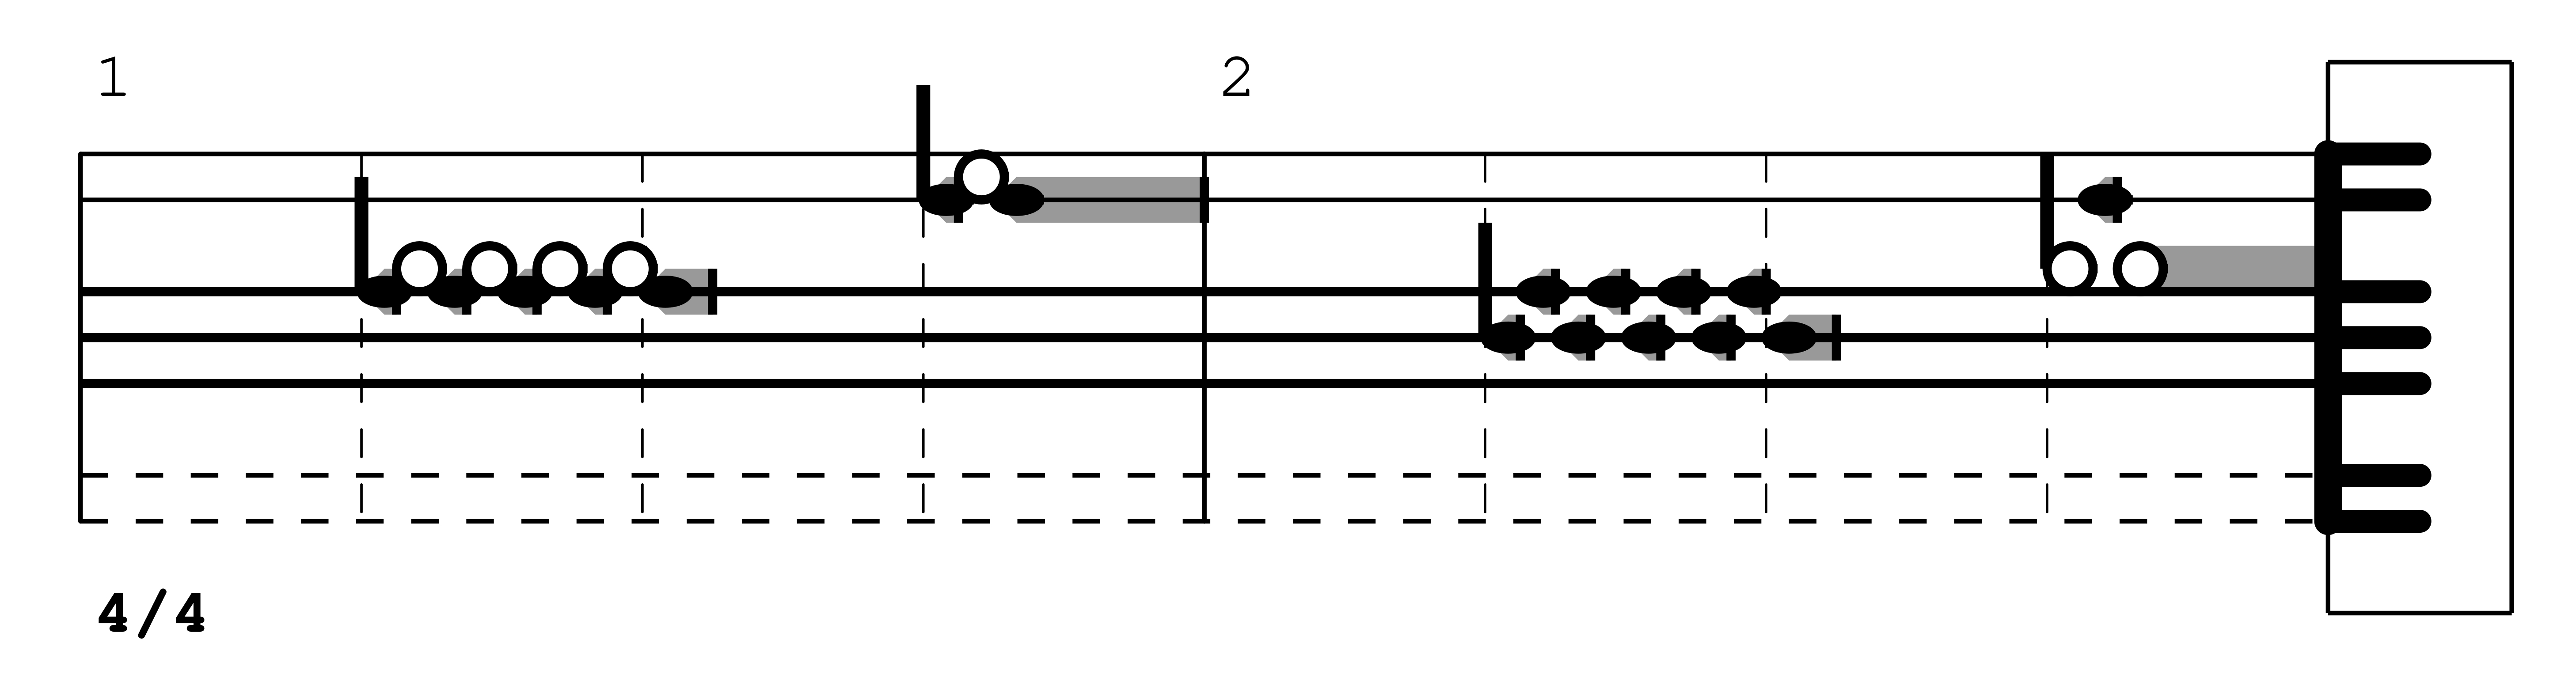
\includegraphics[scale=.75]{images/trills.jpg}\\
\emph{\small picture 4: example of multiple types of trills} 
\end{center}

The first note of an ornament is always written with a stem to give the exact point in time where the base note of the ornament starts.

\subsubsection{Turn}
\begin{center}
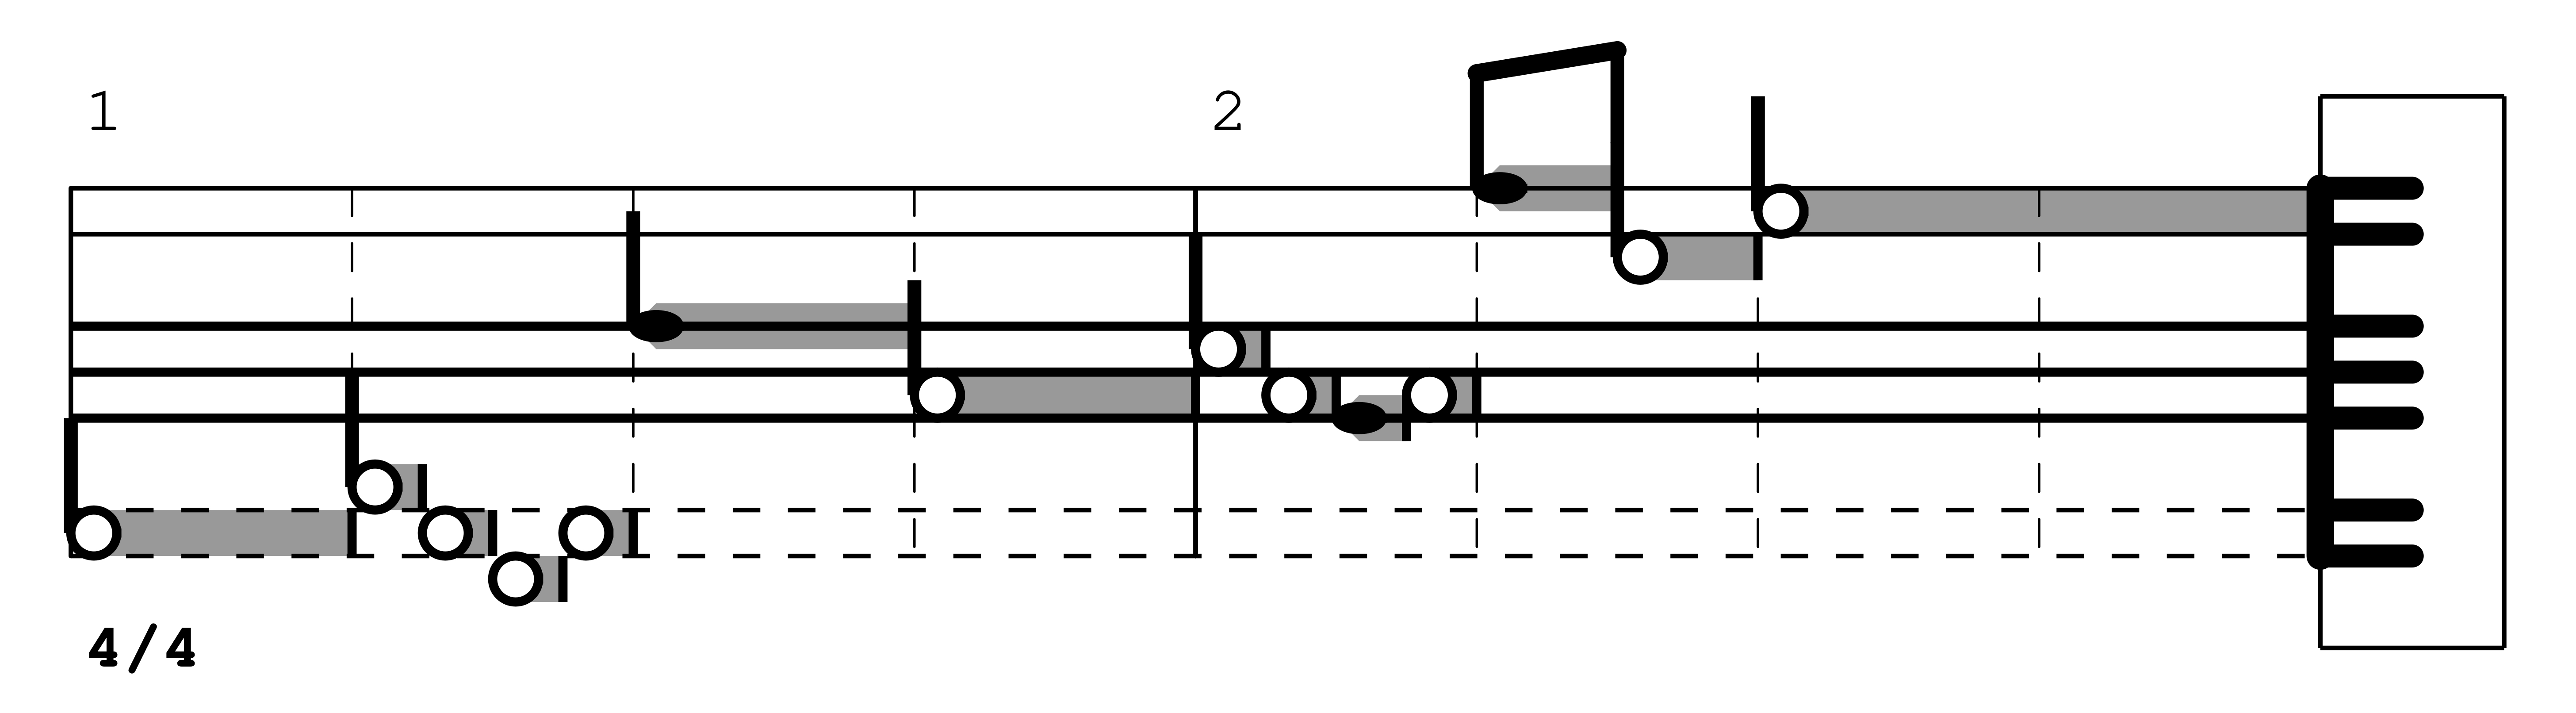
\includegraphics[scale=.75]{images/turns.jpg}\\
\emph{\small picture 5: example of turns in classical music} 
\end{center}

In the above example are two 'turns' in bar 1, second beat, and bar 2, first beat. A turn in traditional music notation is normally written as the middle note of the turn with the turn symbol above it. However, In PianoScript we write it exactly as how you should play a turn since that is the most straight forward way of writing it down.

%------------------------------------------------------------
\subsection{Chords}
Of course, chords should be readable in a clear way. The form of the black notes is slightly different from white notes to be able to read every chord easily.
\begin{center}
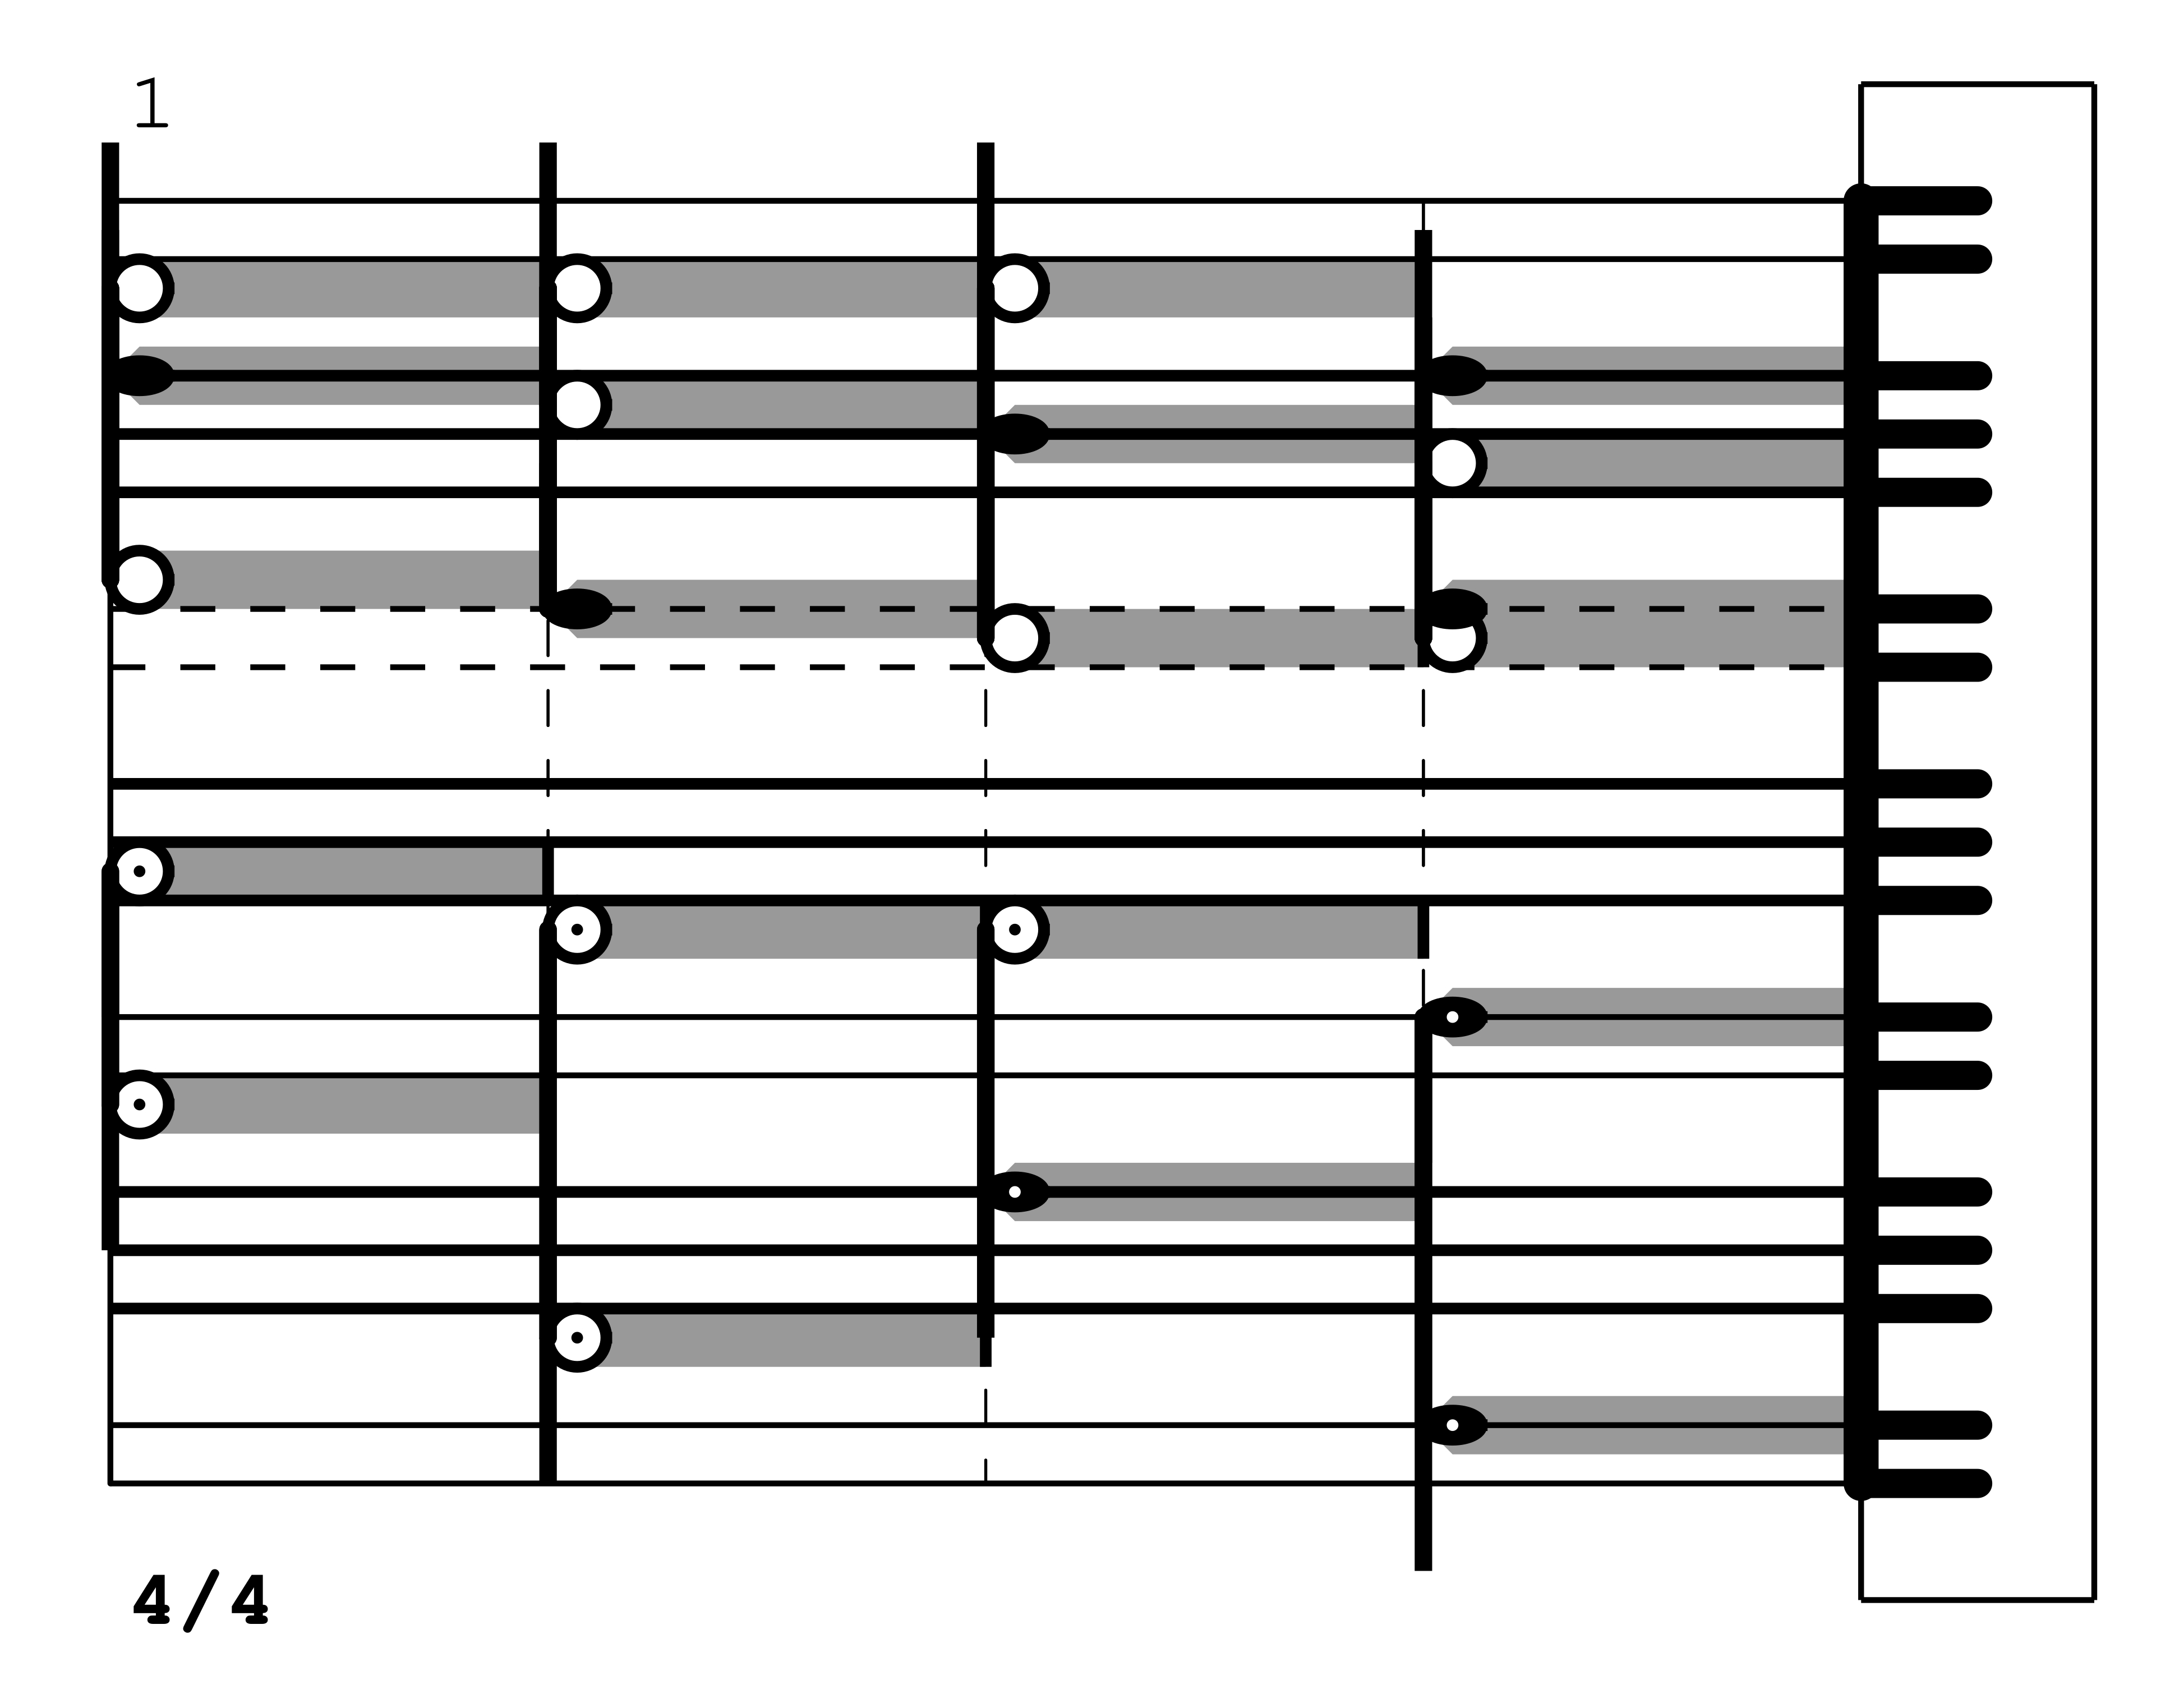
\includegraphics[scale=.75]{images/chords.jpg}\\
\emph{\small picture 6: example of four chords} 
\end{center}

The black notes are twice as small in height and also printed on top of the white notes. In the fourth chord, we see on the right-hand notes an \underline{e\musFlat maj7} chord where the \underline{d} and \underline{e\musFlat}\space are 'glued' together\footnote{In Klavarskribo the black notes are drawn before the stem to prevent collisions. PianoScript does this differently to ensure a constant symbol distance between notes for example in the case of a fast melody.}.

%------------------------------------------------------------
\subsection{Different voices}
In general, you can easily figure out what the different voices are in a piece of harmony:
\begin{center}
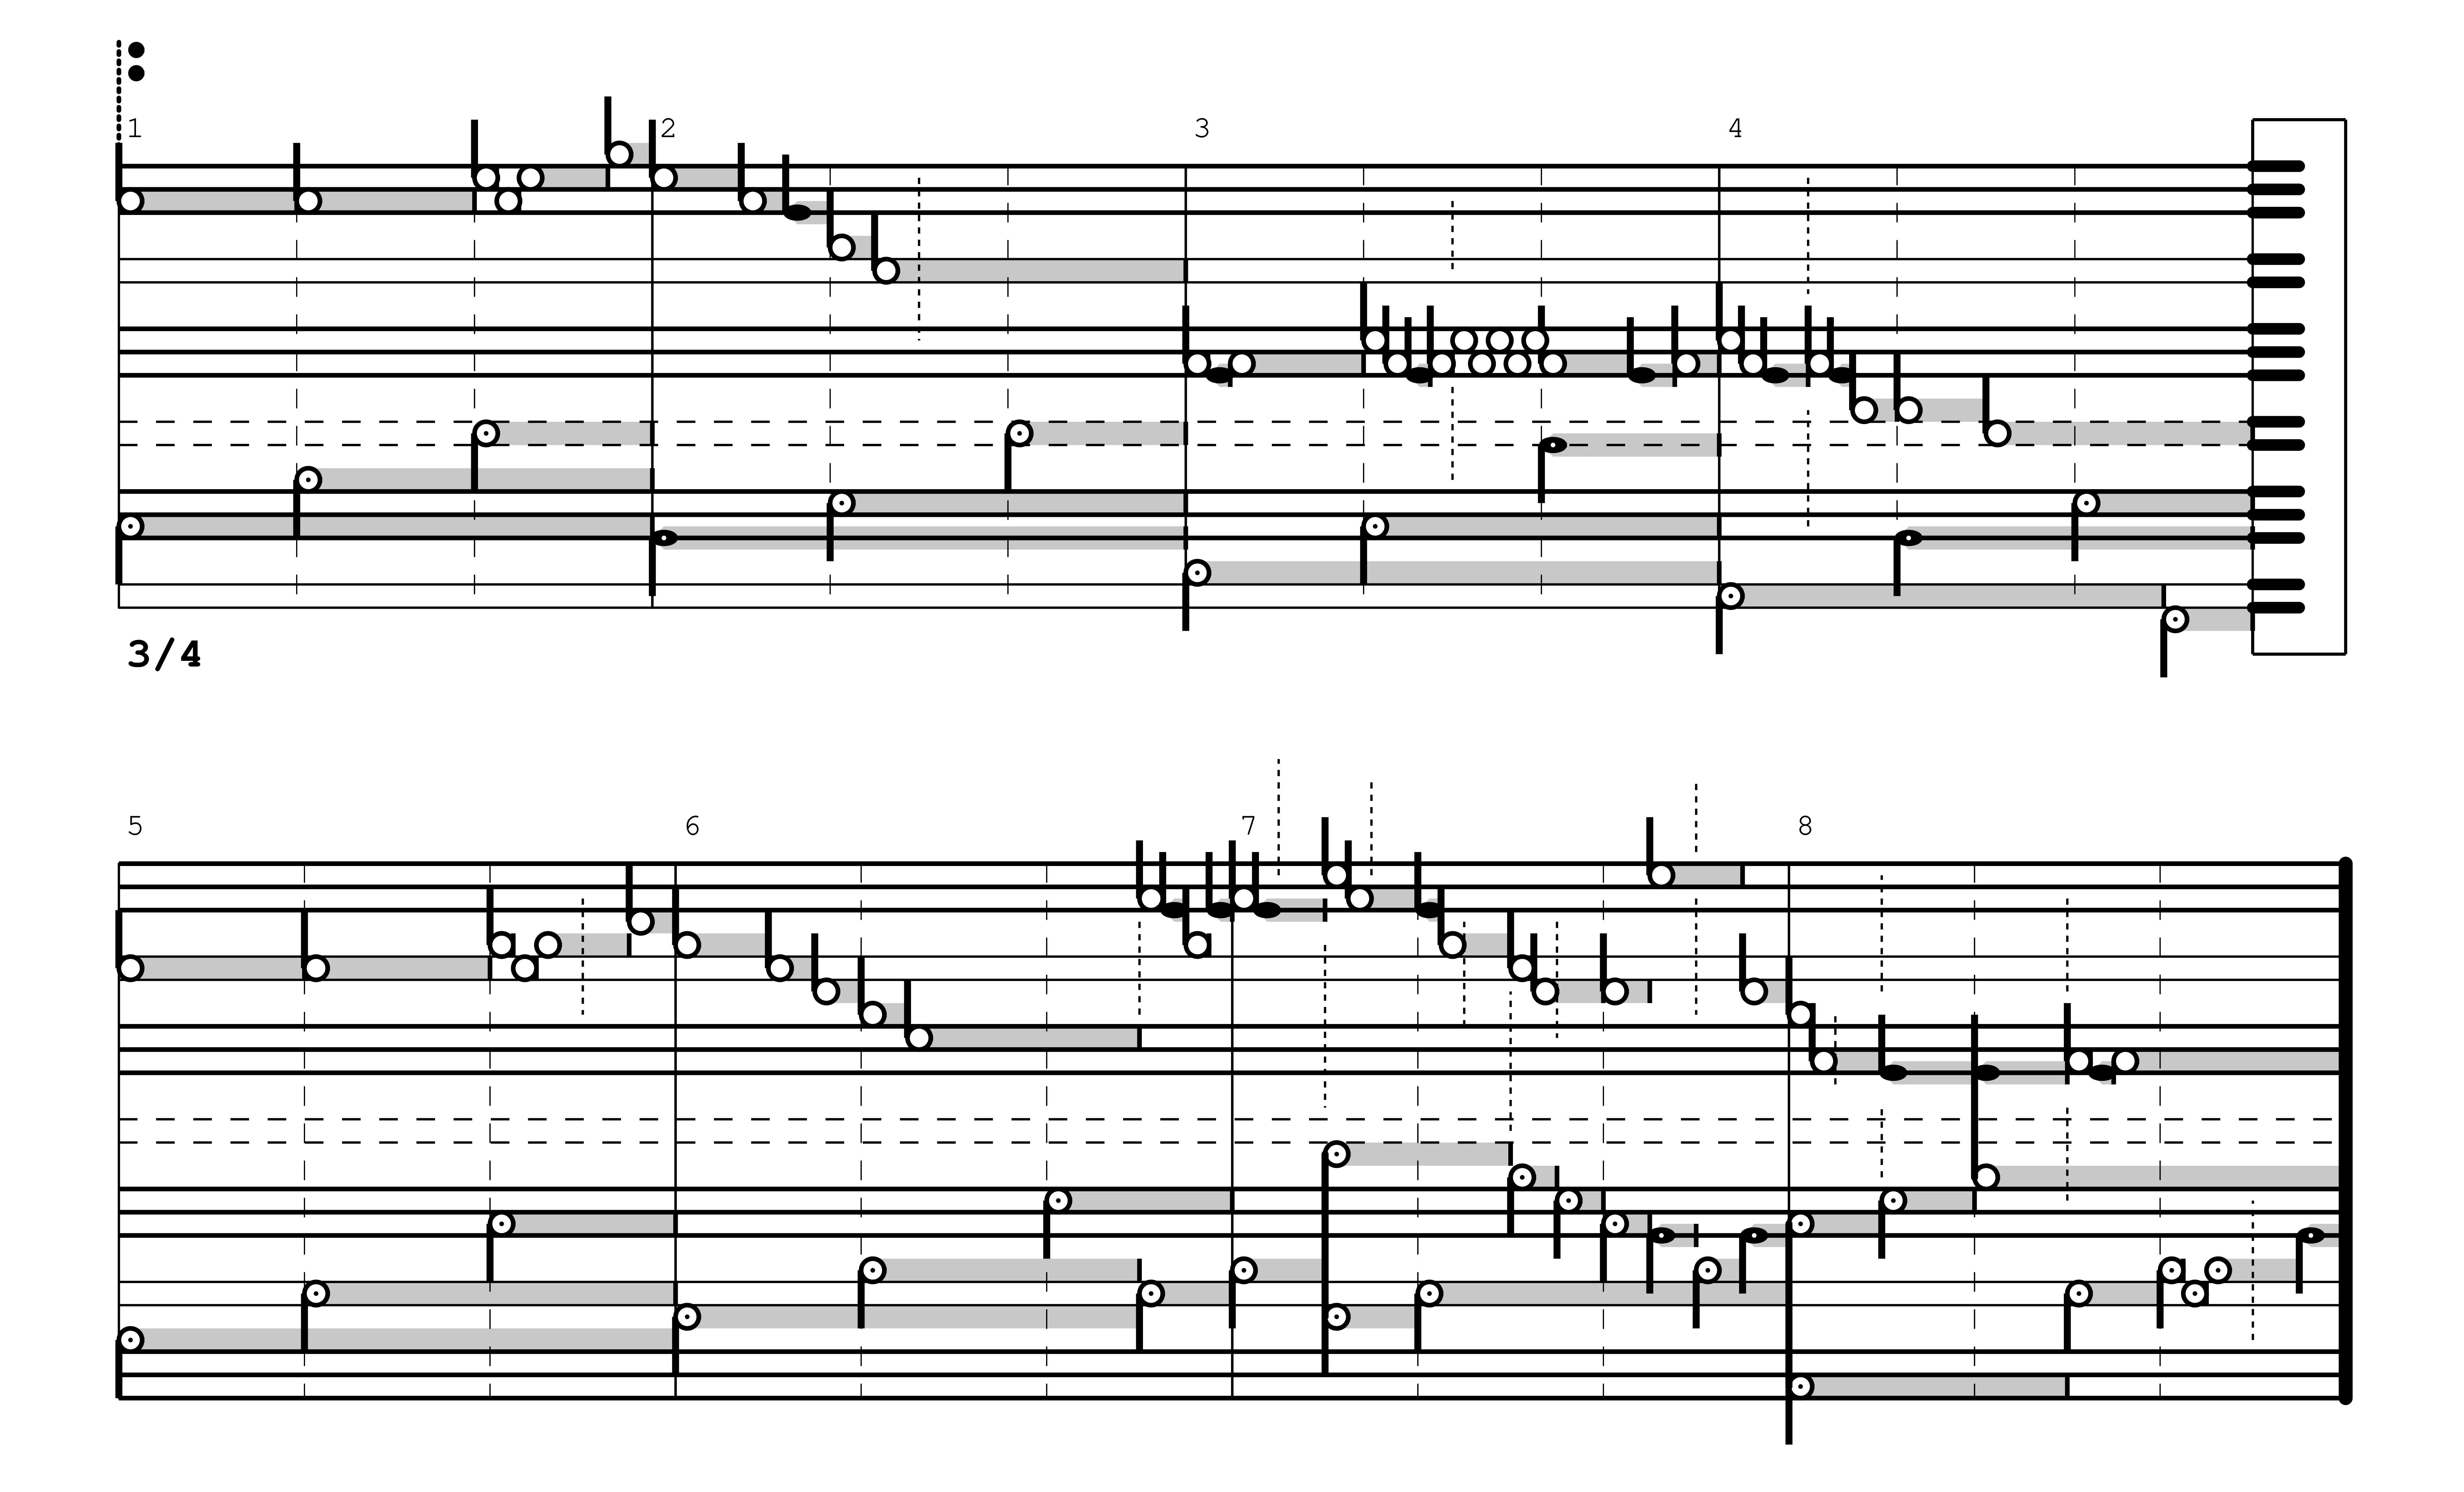
\includegraphics[width=1\textwidth]{images/goldberg.jpg}\\
\emph{\small picture 7: the first eight bars of the goldberg aria by j.s. bach\footnote{the full sheet is at section example sheets}} 
\end{center}
In this example are multiple voices in the left hand. By looking to the harmony you can already figure out where the voices are splitting, stopping or joining. For example in bar 6, left hand, we can visually see how the \underline{c3} and \underline{e3} are joining to a \underline{d3}. In bar 7, left hand, we see how \underline{e3} is splitting into \underline{c3} and \underline{c4}.



%------------------------------------------------------------
\pagebreak
\part{PianoScript software}
\section{Introduction}
PianoScript Score Writer is a python gui program that let's you create full scores in PianoScript format.
\end{document}
